\section{Lösungsansätze in Big-Data Umgebungen}

Im Big-Data Umfeld wurden die Grenzen relationaler Datenbanken früh erkannt und an entsprechenden Lösungsansätzen gearbeitet. Als größtes Hindernis wurde Distanz zum relationalen Datenmodell und deren strikten Einschränkungen geschaffen.

\subsection{NoSQL - flexibel und skalierbar}

Der Begriff NoSQL beschreibt eine Familie von Datenbanken, die sich von dem traditionellen relationalen Datenbankmodell abgrenzen. In der Literatur wird dieser typischerweise als \enquote{not only SQL} interpretiert, entgegen der intuitiven Übersetzung \enquote{kein SQL}. Der Unterschied zu relationalen Datenbanken liegt in der Art der Datensepicherung: Anstelle eines fest definierten Schemas bieten NoSQL-Datenbanken eine flexible Struktur. Grundsätzlich wird zwischen vier Typen von NoSQL-Datenmodellen unterschieden.\footcite[S. 1 f.]{schreinerWhenRelationalBasedApplications2019}

\begin{enumerate}[nosep]
    \item \textbf{Schlüssel-Wert-Datenbanken} speichern Daten als Paarungen aus einem eindeutigen Schlüssel und einem zugehörigen Wert. Der Schlüssel dient zur Identifizierung des Werts, ähnlich wie ein Primärschlüssel in RDBMS. \footcite[S. 2]{wangSQLVsNoSQL2017}
    \item \textbf{Spaltenorientierte Datenbanken} speichern Daten in Spaltenfamilien statt, wie bei RDBMS üblich, in Zeilen. Zusammengehörige Daten werden aggregiert gespeichert und ermöglichen hohe Skalierbarkeit durch Verteiliung der unterschiedlichen Spaltenfamilien auf verschiedene Knoten. \footcite{}
    \item \textbf{Dokumentorientierte Datenbanken} verwalten Daten in flexiblen, hierachisch strukturierten Dokumenten, meist im JSON-Format. Jedes Dokument kann eine unterschiedliche Struktur aufweisen, wodurch dynamische und variable Datenmodelle untersützt werden.
    \item \textbf{Graphdatenbanken} speichern Daten als Knoten und deren Beziehungen als Kanten. Vernetzte Datenstrukturen, bei denen die Beziehungen zischen Datenelementen im Vordergrund stehen, können in Graphdatenbanken effizient abgebildet werden. \footcite{}
\end{enumerate}

Die ersten drei Datenbanktypen unterscheiden sich in ihrer Art, stark von den Graphdatenbanken. Fowler schlägt daher die Teilung der NoSQL-Familie  in zwei übergreifende Kategorien vor: Die Aggregat-orientierten Datenbanken, speichern zusammengehörige gemeinsam ab. Hier ist der Unterschied zu relationalen Datenbanken erkennbar, wo zusamenhängende Daten meist durch die Normalisierung auseinandergerissen werden. Graphdatenbanken hingegen, sind spezialisiert auf die noch stärkere Verteilung von Daten welche nicht im direkten Zusammenhang zueinander stehen, sondern lediglich in Bestimmten Situationen oder Anwendung in Verbindung oder Beziehung zueinander stehen. \footcite{fowlerAggregateOrientedDatabase2012}

\subsection{Fallbeispiel: Polyglot Persistence}

Die Wahl eines geeigneten Datenbanksystems war in der Vergangenheit unkompliziert, da sie sich ausschließlich auf die Entscheidung für eines der verfügbaren relationalen Datanbanksystems beschränkte. Mit dem Aufkommen von NoSQL-Datenbanken wurde diese Entscheidung jedoch deutlich komplexer. Neben der grundlegenden Wahl zwischen relationalen und nicht-relationalen Datenbanken muss nun auch innerhalb der NoSQL-Landschaft zwischen verschiedenen Datenbanktypen abgewogen werden. Zudem spielt die Erfahrung der Entwickelnden eine größere Rolle, da NoSQL-Datenbanken meist keine universelle Abfragesprache wie SQL unterstützen. Während relationale Datenbanken für die Mehrheit der Anwendungen mit strukturierten Daten weiterhin die bevorzugte Wahl darstellen, gibt es Szenarien, in denen NoSQL-Lösungen besser geeignet sind. \footcite[S. 194]{harrisonNextGenerationDatabases2015} Der Einsatz verschiedener Datenbanktypen für verschiedene Anwendungsfälle wird als \textbf{Polyglot Persistence} bezeichnet. Das von \textit{Fowler} popularisierte Architekturmuster steht kontrastierend zum \textit{\enquote{one-size-fits all}}-Prinzip, das eine monolithische und anwendungsübergreifende Datenbankarchitektur anstrebt. Stattdessen verfolgt Polyglot Persistence das Ziel, für jede Anwendung die am besten geeigneten Datenbanksysteme zu wählen. Vorteile sind die gesteigerte Produktivität und die Reduktion des Impedance Mismatch. Beispielsweise eignen sich Dokumentendatenbanken besonders für die Persistierung komplexerer und semi-strukturierter Objekte, während für strukturierte Daten weiterhin die Vorteile relationaler Datenbanken genutzt werden können. \footcite[S. 1 f.]{gessertPolyglotPersistence2015} Abbildung 1 skizziert die Datenbankarchitektur einer E-Commerce Plattform basierend auf der Polyglot-Persistence.

\begin{figure}[H]
    \centering
    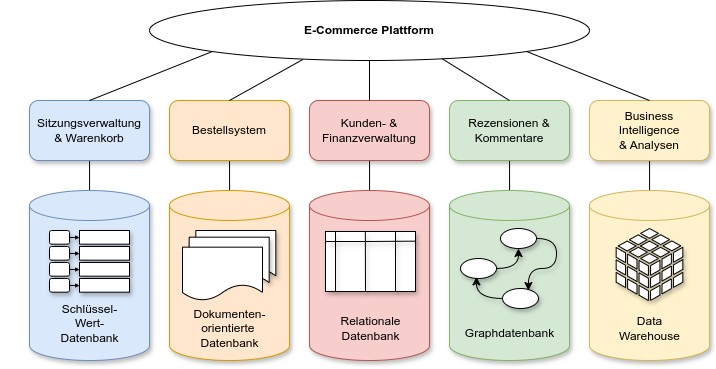
\includegraphics[width=0.9\textwidth]{online-shop-db-architecture.png}
    \caption{Beispielhafte Datenbankarchitektur einer modernen und skalierbaren E-Commerce Plattform. In Anlenung an \cite{donofrioBigDataAnalytics2021}.}
    % \footcite[S. 7]{meierWerkzeugeDigitalenWirtschaft2018}
\end{figure}

Erkennbar ist, das für die unterschiedlichen Funktionen verschiedene Datenbankmodelle gewählt wurden. Für die Verwaltung der Nutzersitzungen und Warenkörbe könnte eine einface Schlüssel-Wert-Datenbank sinnvoll sein, da sie hohe Verfügbarkeit und Ausfalltoleranz gewährleistet. Das Bestellsystem erfordert ebenfalls hohe Verfügbarkeit sowie Flexibilität und Skalierbarkeit, weshalb die Verwendung eines Dokumentenspeichers in Betracht zu ziehen ist. Die Verwaltung von Kundendaten und Transaktionen in der Finanzverwaltung stellt hohe Anforderungen an Konsistenz, weshalb relationale Datenbanken mit ihren ACID-Eigenschaften besonders geeignet erscheinen. Bei Produktrezensionen, Kommentaren und Interaktionen handelt es sich um vernetzte Daten, für die sich eine Graphdatenbank anbietet, da sie gezielte Auswertungen von Kundenbeziehungen ermöglicht. Für Business-Intelligence-Aufgaben wie Aggregationen, Analysen und die Bereitstellung aktueller Kennzahlen empfiehlt sich der Betrieb eines Data Warehouses. \footcite[S. 8]{donofrioBigDataAnalytics2021} \vspace{0.1cm} \footcite[S. 47]{meierWerkzeugeDigitalenWirtschaft2018}

% Hierfür kommt beispielsweise eine In-Memory Spaltenfamielendatenbank in Frage, welche die notwendige Performance und Flexibilität vereinigt.

% Polyglot Persitstance !!!

% \subsection{Zurück zu SQL - NewSQL}
% \subsection{Zurück zu (New)SQL}
% \subsection{NewSQL \& die Zukunft von Datenbanken}
\subsection{NewSQL \& Die Datenbanken der Zukunft}

% Das zweite Kapitel dieser Arbeit behandelte bereits ausführlich die Limitierungen RDBMS, insbesondere in den domänenspezifischen Anforderungen von BigData. Dennoch bleiben relationale Datenbanken trotz ihrer Nachteile weiterhin weit verbereitet. Ein wesentlicher Grund dafür dürfte die Abfragesprache SQL sein. Als universelle, datenbankübergreifende Sprache auf Basis des relationalen Modells bietet sie einen entscheidenden Vorteil, der viele der bekannten Einschränkungen ausgleicht.
% Demgegenüber steht die fragmentierte NoSQL-Landschaft, in der jede Datenbankimplementierung eigene Syntax- und Grammatiksprachen verwendet. Diese uneinheitliche Abfragesituation erwies sich als hinderlich für die Akzeptanz und breite Durchsetzung von NoSQL-Systemen. 

% In den letzten Jahren wurden daher verstärkt Forderungen nach einer erneuten Standardisierung von Abfragesprachen laut. Neue Datenbanken sollten die Vorteile der NoSQL-Ära mit den Stärken relationaler Systeme kombinieren. Dieser Ansatz wird als NewSQL bezeichnet und beschreibt den Trend zurück zu SQL oder SQL-ähnlichen Abfragesprachen, kombiniert mit der Skalierbarkeit und Flexibilität moderner Datenbanksysteme. 

% Während Polyglot Persistence eine Möglichkeit bietet, die Vorteile verschiedener Datenbanktypen zu kombinieren, bringt dieser Ansatz auch Herausforderungen mit sich. Dazu zählen die Wahl der optimalen Datenbank für einen spezifischen Anwendungsfall sowie Konsistenzprobleme, die sich aus den Unterschieden zwischen Datenbankmodellen und Abfragesprachen ergeben. \footcite[S. 3 f.]{gessertPolyglotPersistence2015} Die ideale Lösung wäre eine Brücke zwischen RDBMS und NoSQL-Systemen, welche die jeweiligen Stärken beider Technologien vereint. Ein solcher Ansatz existiert bereits unter dem Begriff \textbf{NewSQL} und beschreibt den Trend zu relationalen Datenbanken, die Skalierbarkeit und Flexibilität moderner NoSQL-Technologien integrieren. Obwohl sich reine NewSQL-Datenbanken bislang nicht flächendeckend durchsetzen konnten, argumentieren \textit{Stonebraker und Pavlo}, dass sie maßgeblich zur zunehmenden Konvergenz zwischen relationalen und nicht-relationalen Datenbanken beigetragen haben. Insbesondere zeigte NewSQL, dass sich verteilte NoSQL-Architekturen mit ACID-Eigenschaften kombinieren lassen. \footcite[S. 29 ff.]{stonebrakerWhatGoesComes2024} 

% Anstelle eines Kompromisses zwischen verschiedenen, untereinander inkompatiblen Technologien skizziert \textit{Harrison (2015)} die Datenbank Zukunft: ein einheitliches System, das sich flexibel an unterschiedliche Anforderungen und Datenformate anpassen kann. Ein solches Modell müsste sowohl die Normalform relationaler Systeme als auch die Speicherung dynamischer und komplexer Objektstrukturen in Form von Dokumenten ermöglichen. \footcite[S. 195-20, S. 214]{harrisonNextGenerationDatabases2015} 
% Heute sind wir dieser Vision näher denn ja. Die Mehrheit der NoSQL-Datenbanken setzt mittlerweile verstärkt auf konsistente ACID-Transaktionen und bietet SQL- kompatible Schnittstellen an. Gleichzeitig adaptieren RDBMS zunehmend Konzepte des nicht-relationalen Modells und unterstützen inzwischen mehrheitlich die Speicherung von Schlüssel-Wert-Paaren oder gesamten Dokumentstrukturen im JSON-Format. \footcite[S. 22 ff.]{stonebrakerWhatGoesComes2024} Während die Grenzen zwischen RDBMS, NoSQL und NewSQL zunehmend verschwimmen, bleibt das relationale Modell sowie SQL, angereichert mit neuen Funktionen und Konzepten, die einzige Konstante – ganz nach dem Motto:

% \textit{„What Goes Around Comes Around... And Around...“} \footcite[S. 32]{stonebrakerWhatGoesComes2024}

Während Polyglot Persistence eine Möglichkeit bietet, die Vorteile verschiedener Datenbanktypen zu kombinieren, bringt dieser Ansatz auch Herausforderungen mit sich. Dazu zählen die Wahl der optimalen Datenbank für einen Anwendungsfall sowie Konsistenzprobleme durch unterschiedliche Datenmodelle und Abfragesprachen. \footcite[S. 3 f.]{gessertPolyglotPersistence2015} Die ideale Lösung wäre eine Brücke zwischen RDBMS und NoSQL-Systemen, die die jeweiligen Stärken beider Technologien vereint. Ein solcher Ansatz existiert bereits unter dem Begriff NewSQL und beschreibt relationale Datenbanken, die Skalierbarkeit und Flexibilität moderner NoSQL-Technologien integrieren. Obwohl sich reine NewSQL-Datenbanken noch nicht durchsetzen konnten, argumentieren Stonebraker und Pavlo, dass sie die Konvergenz zwischen relationalen und nicht-relationalen Systemen vorangetrieben haben. Insbesondere zeigte NewSQL, dass sich verteilte NoSQL-Architekturen mit ACID-Eigenschaften kombinieren lassen. \footcite[S. 29 ff.]{stonebrakerWhatGoesComes2024}

Anstelle eines Kompromisses zwischen inkompatiblen Technologien skizzierte Harrison (2015) die Datenbank der Zukunft als ein einheitliches System, das sich flexibel an verschiedene Anforderungen anpassen kann. Ein solches Modell müsste sowohl die Normalform relationaler Systeme als auch die Speicherung komplexer Objektstrukturen in Dokumenten ermöglichen. \footcite[S. 195–202, S. 214]{harrisonNextGenerationDatabases2015} Heute sind wir dieser Vision näher denn je: NoSQL-Datenbanken setzen zunehmend auf ACID-Transaktionen und bieten SQL-kompatible Schnittstellen. Gleichzeitig adaptieren RDBMS Konzepte des nicht-relationalen Modells und unterstützen die Speicherung von Schlüssel-Wert-Paaren und Dokumentstrukturen. \footcite[S. 22 ff.]{stonebrakerWhatGoesComes2024} Während Multi-Modell-Datenbanken die Grenzen zwischen RDBMS, NoSQL und NewSQL zunehmend auflösen, bleibt das erweiterte relationale Modell in Verbindung mit modernem SQL als zentrale Konstante bestehen – gemäß dem Prinzip: 

\begin{center}
    \textit{„What Goes Around Comes Around... And Around...“} \vspace{0.1cm}\footcite{stonebrakerWhatGoesComes2024}
\end{center}

% was dazu führte, dass viele große NoSQL-Datenbanken inzwischen konsistente Transaktionsmodelle und übernommen haben. Gleichzeitig haben moderne relationale Datenbanken 


% Solche Datenbanken würden die Vorteile von NoSQL mit den von RDBMS kombinieren. Dieser Ansatz exisitiert und wird oft als NewSQL bezeichnet und beschreibt den Trend hin zu relationalen Datenbanken mit der Skalierbarkeit und Flexibilität moderner NoSQL-Technologien. Reine NewSQL Datenbanken konnten sich bis heute nicht durchsetzen, Stonebraker und Pavlo argumentieren argumentieren jedoch dass sie maßgeblich Verantwortlich waren für die in den letzten Jahren zunehmende Konvergenz relationaler und nicht-relationaler Datenbanken. NewSQL zeigte dabei die Vereinbarkeit verteilter NoSQL-Datenbanken mit den ACID-Eigenschaften auf, was zu der Verbreitung dieser Eigenschaften in den größten NoSQL Datenbank führte.


% Anstelle eines Kompromisses zwischen verschiedenen untereinander inkompatiblen Technologien skizziert Harrison im Jahr 2015 die Datenbank Zukunft: ein einheitliches System, das sich flexibel an unterschiedliche Anforderungen und Datenformate anpassen kann. Ein solches Modell müsste heterogene Datenstrukturen unterstützen und sowohl die Normalform relationaler Systeme als auch die Speicherung dynamischer und komplexer Objektstrukturen in Form von Dokumenten ermöglichen. \footcite[S. 195-20, S. 214]{harrisonNextGenerationDatabases2015}  

% Statt dem Kompromiss zwischen verschiedenen inkompatiblen Technologien zeichnet Harrison in seinem letzten Kapitel das Bild der Datenbank der Zukunft: Ein einheitliches Datenbanksystem welches an die jeweiligen Anforderungen und Datenformate verschiedenster Anwendungen angepasst werden kann. Ein solches Datenmodell müsste dabei Daten unterschiedlicher Formate unterstützen. Die Datenbank würde somit gleichzeitig die Normalform des relationalen Modells sowie die Speicherung dynamischer und komplexen Objektstrukturen als gesamtes Dokument ermöglicht.

% \textit{Michael Stonebraker} und \textit{Andrew Pavlo} fassen diese Entwicklungen treffend in ihrem Artikel \textit{\enquote{What Goes Around Comes Around... And Around...}} aus dem Jahr 2024 zusammen. \footcite{stonebrakerWhatGoesComes2024}